\section{Mass and Inertia from Vortex Circulation}

In the Vortex Æther Model (VAM), mass is not a fundamental attribute but emerges from fluid motion—specifically the swirl dynamics and circulation of knotted vortex structures. This section derives the mass-energy relation, effective inertial mass, and corresponding Lagrangian term based purely on ætheric fluid mechanics.

\subsection{Kinetic Energy of a Vortex Knot}

The kinetic energy of a localized vortex knot in an incompressible æther is given by:
\begin{equation}
    \mathcal{L}_\text{kin} = \frac{1}{2} \rho_\text{\ae} |\vec{v}|^2,
\end{equation}
where $\vec{v}$ is the swirl velocity and $\rho_\text{\ae}$ the local æther density. For a stable vortex knot, the core swirl velocity saturates at a characteristic value \( C_e \), yielding:
\[
    \mathcal{L}_\text{kin} \approx \frac{1}{2} \rho_\text{\ae} C_e^2.
\]
Assuming a knot core with radius \( r_c \), the total kinetic energy becomes:
\[
    E_\text{kin} \approx \frac{1}{2} \rho_\text{\ae} C_e^2 \cdot \frac{4}{3} \pi r_c^3.
\]
This naturally defines an effective inertial mass:
\[
    m_\text{eff} = \rho_\text{\ae} \cdot \frac{4}{3} \pi r_c^3,
    \qquad \Rightarrow \qquad E = \frac{1}{2} m_\text{eff} C_e^2.
\]

\subsection{Circulation and Geometric Mass Emergence}

In vortex mechanics, circulation is conserved and fundamental. It is defined as:
\begin{equation}
    \Gamma = \oint_{\partial S} \vec{v} \cdot d\vec{\ell} = 2\pi r_c C_e.
\end{equation}
This relation implies that any deformation in core radius \( r_c \) demands a reciprocal change in swirl velocity \( C_e \), preserving $\Gamma$ and enforcing inertial resistance.

We now compute the full kinetic energy from this identity:
\begin{align}
    E &= \frac{1}{2} \rho_\text{\ae} \left( \frac{\Gamma}{2\pi r_c} \right)^2 \cdot \frac{4}{3} \pi r_c^3
      = \frac{\rho_\text{\ae} \Gamma^2}{6\pi r_c}.
\end{align}
Comparing with \( E = \frac{1}{2} m C_e^2 \), we extract the effective mass:
\begin{equation}
    m_\text{eff} = \frac{\rho_\text{\ae} \Gamma^2}{3\pi r_c C_e^2}.
\end{equation}
This demonstrates that mass is not an input parameter but a derived quantity—arising from æther density, core geometry, and topological circulation.

\subsection{Lagrangian Mass Term in VAM}

Given the above, the corresponding mass term for a fermion field $\psi_f$ is:
\begin{equation}
    \mathcal{L}_\text{mass} = m_f C_e r_c \cdot \bar{\psi}_f \psi_f,
\end{equation}
where \( \hbar_\text{VAM} = m_f C_e r_c \) acts as an emergent angular momentum scale. This replaces the conventional Yukawa interaction with a mechanical origin grounded in vortex dynamics.

\begin{figure}[H]
    \centering
    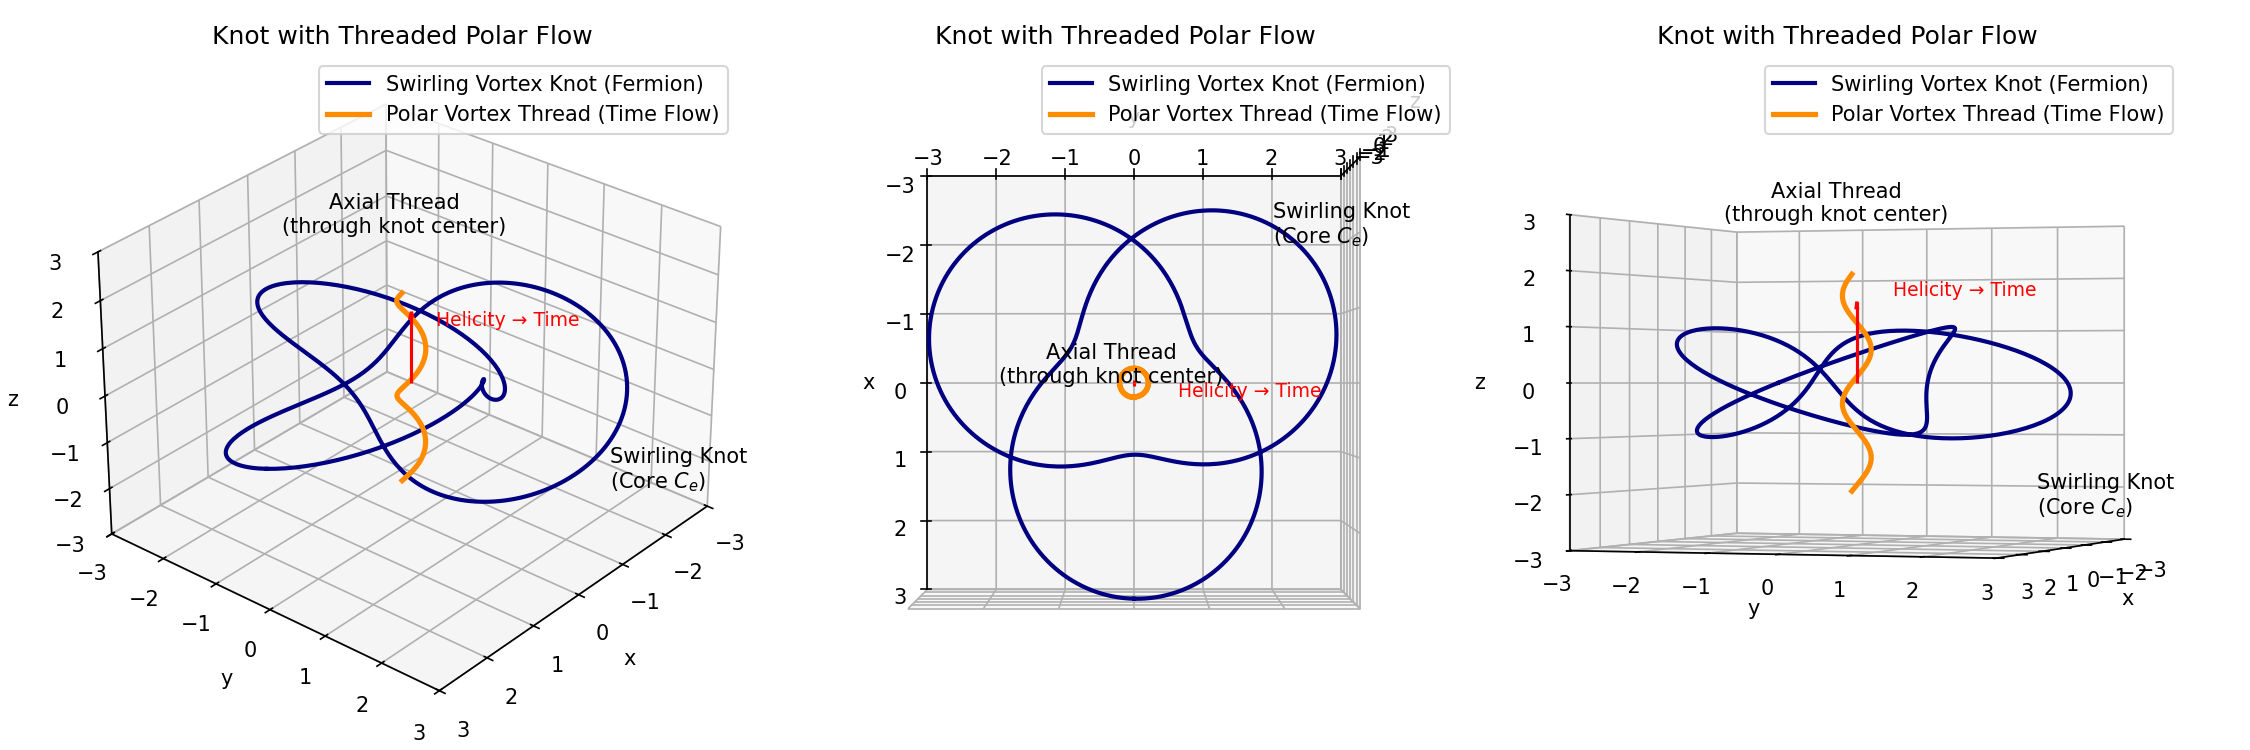
\includegraphics[width=0.95\textwidth]{KnotThreadedPolarFlow.png}
    \caption{Topological vortex knot with helicity axis and circulation scale \( \Gamma = 2\pi r_c C_e \). The axial outflow encodes the emergent time direction.}
\end{figure}

This unification of mass, energy, and time within the same geometric vortex structure lays the foundation for subsequent reformulation of spin, field interactions, and temporal flow in the next sections.
